%************************************************
\chapter{Patterns of sitewise selection in mammalian protein-coding genes}\label{ch:mammals1}
%************************************************

\section{Introduction}

\subsection{The Mammalian Genome Project}

A major goal of mammalian comparative genomics has been to quantify,
identify and understand the fraction of the human genome that is under
evolutionary constraint. The first non-human mammalian genomes showed
at least 5\% of the human genome to be under purifying selection
\citep{Mouse2002Initial,Rat2004Genome,LindbladToh2005Genome}, but the
small number of genomes available limited the extent to which regions
of evolutionary constraint could be identified. The \mgp, a
coordinated set of genome sequencing projects initiated in 2005 and
organised by the Broad Institute of MIT and Harvard, was designed with
the primary purpose of increasing the accuracy and confidence with
which regions of the human genome that have evolved under evolutionary
constraint in mammals could be identified \citep{TODO}. In line with
this goal, 20 mammalian species were chosen for sequencing in order to
maximise the amount of evolutionary divergence available for
comparative analysis when combined with the 9 already available
sequenced genomes \citep{Margulies2005Initial}. To save on sequencing
costs most of the 20 additional species were only sequenced to a
target twofold coverage, meaning each genomic base pair would be
covered on average by two sequence reads and roughly 85\% of genomic
sequence would be covered by at least one read.

As the \mgp proceeded from its sequencing to analysis phase in late
2008, it became clear that the additional branch length afforded by
the 29-species phylogeny would enable a number of improved
evolutionary analyses beyond the identification of constrained
noncoding regions. Among others, these included the evolutionary
characterisation of gene promoters, identification of exapted
noncoding elements, detection of evolutionary acceleration and
deceleration in noncoding regions, and detection of purifying and
positive selection in protein-coding genes. Given its prior
involvement in analysing the ENCODE comparative sequencing data
\citep{TODO} and Massingham's work on a method and software program
for sitewise evolutionary analysis \citep{TODO}, the Goldman group
became involved in the protein-coding evolutionary analysis for the
\mgp. This chapter describes my work on the project, which began in
late 2008; the major results from the analysis are to be published in
\citep{TODO}, and all of the work described below was performed by me
in consultation with members of the Goldman group (Nick Goldman and
Tim Massingham), EnsEMBL team (Albert Vilella, Javier Herrero, Ewan
Birney) and organisers and members of the \mgp (Manolis Kellis,
Kerstin Lindblad-Toh, Mike Lin, Katie Pollard).

\subsection{The Sitewise Likelihood Ratio test}

As described in Chapter \ref{ch_bg}, differential survival of \nsyn
and \syn mutations based on the degeneracy of the genetic code can be
used as a source of information on the continued importance of
mutations at a given protein-coding site over evolutionary time: a
lower rate of \nsyn substitution compared to \syn substitution is
indicative of purifying selection, or natural selection in favor of
maintaining protein structure and function; equal rates of \nsyn and
\syn substitutions is indicative of neutral selection, or no
differential survival of protein-altering mutations; a greater rate of
\nsyn than \syn substitution is indicative of positive selection, or
natural selection in favor of protein-altering mutations.

Early evolutionary analyses of protein sequences showed large
variation in the rates of amino acid change both within and between
proteins \citep{TODO}. This variety results from the myriad structures
and functions embodied by different proteins and protein domains
\citep{TODO}. Continued work suggested that the overall evolutionary
rate \cite{TODO,Koonin?} and the pattern of localised selective
pressures \cite{TODO} of a gene can reveal important insight into its
role in the organism. Thus, the study of rates of \nsyn and \syn
substitution in proteins became established as an effective method for
using evolutionary information to investigate the functional
characteristics of genes.

Maximum likelihood methods, introduced in Chapter \ref{TODO}, are
commonly applied to biological sequence analysis due to their
desirable statistical features...

The Sitewise Likelihood Ratio (SLR) test is based on the mechanistic
Goldman-Yang codon model of evolution, with an additional parameter
for each site in the alignment representing the sitewise $\omega$
value. The inclusion of an additional parameter per alignment site
makes the model extremely complex and difficult to optimise, but the
dimensionality of the likelihood optimisation is reduced by making the
assumption that the $\omega$ at each site does not contribute
significantly to the overall likelihood, thus allowing for separate
optimisation of the global parameters (including XYZ) across the whole
alignment and the $\omega$ parameter at each site. In this way, SLR
performs an approximate likelihood ratio test (LRT) for non-neutral
evolution at each site...

\subsection{Data quality concerns: alignment and sequencing error}

The possibility that errors in the source alignments might cause false
positives in the detection of sitewise positive selection was a major
concern for this analysis. Although the SLR test and other \sw \ml
methods have been shown to be conservative for detecting positive
selection even when the amount of data is low or the null model is
violated \citep{Anisimova2002Properties,Massingham2005Detecting,TODO},
most evolutionary analyses are based on the assumption that all sites
within an alignment column are truly homologous. This assumption can
be violated in a number of ways, some of which are described below.

Alignment error results from the difficulty of reconstructing the
evolutionary history of sequences evolving with indels and can cause
nonhomologous codons to be placed in the same alignment column. In
Chapters \ref{ch_indel1} and \ref{ch_indel2} I explored the tendency
of multiple aligners to produce such errors, showing that \prankc
alignments would be expected to introduce few falsely identified
positively-selected sites resulting from alignment errors at
mammalian-like divergence levels.

Errors resulting from incorrect genomic sequence was an additional
concern. Twenty of the genomes under study were sequenced at low
coverage and were not assembled into chromosomes or finished to
completion, making the likelihood of miscalled bases, spurious
insertions or deletions, or shuffled regions due to misassembly
relatively high \citep{TODO}. The potential effect of each of the
aforementioned types of sequence errors on the detection of positive
or purifying selection depends on the nature of the inference method,
the type of sequencing error, and the branch length of the terminal
lineage leading to the species containing the error.

As most codon-based inference methods assume independence between
amino acid sites, I first consider the effect---in isolation---of a
single spuriously-assigned homologous codon on the \ml estimation of
$\omega$. Two cases can be considered: a single sequence error causing
one spurious substitution within a codon, and one or multiple sequence
or assembly errors causing multiple spurious substitutions within a
codon. In the case of a single spurious substitution, if we assume no
large difference between the natural mutational process and the
process that caused the erroneous mutation, then the effect would be
to shift the estimated $\omega$ in the branch containing the error
towards 1. The sequence error would be incorporated into the \ml
optimisation as an additional neutral substitution, inflating the
estimated substitution rate but not affecting the relative \nsyn and
\syn rates. This effect may be biased towards higher or lower $\omega$
values if a significant difference exists between the neutral
biological mutational process and the pseudo-mutational process
causing the erroneous substitution. On the other hand, a codon with
multiple erroneous bases may cause greater elevation of the inferred
substitution rate and $\omega$, due to the necessity of \ml methods to
infer a multi-step path of single substitutions between the two codons
on either side of a given evolutionary branch. The path estimated
between two completely nonhomologous codons depends on the estimated
codon frequencies, the genetic code, and the pseudo-mutational
process; while a detailed investigation of the expected effect on
inferred $\omega$ values is beyond the scope of my analysis, it is not
unreasonable to expect a greater number of false positive \pss{}s
resulting from codons with multiple erroneous bases than from codons
with single errors.

{\color{red} TODO: quick randomisation experiment looking at elevated
  $\omega$ from multi-substitution codons?}

Given the potentially greater impact of codons with multiple errors,
the propensity of each of the common sequencing error types identified
above (miscalled bases, spurious indels, and
shuffled/repeated/collapsed regions due to mis-assembly) to cause
single or multiple errors within codons could strongly affect its
effect on the detection of positive selection. On its own, a miscalled
base would obviously result in a single spurious
substitution. However, low-quality bases tend not to be uniformly
distributed among or within sequence reads, which makes for a larger
probability of multiple errors within a codon resulting from miscalled
bases. Spurious indels within coding regions may be even more likely
than miscalled bases to cause multiple errors within a codon due to
the potential alignment and frameshift effects (but see the discussion
of Ensembl's frameshift filters for low-coverage genomes in Section
\ref{TODO}). Assembly errors, which result in larger-scale structural
errors including missing, repeated, shuffled or inverted sequence
regions, are most prone to produce codons with multiple erroneous
errors due to the large amount of contiguous sequence data being
misplaced.

I also note the impact of the inference method and terminal branch
length on false positives resulting from sequence errors, which can be
understood in terms of the information most directly affecting the
inference of a positively selected site or a positively selected gene
for a given detection method. Both the branch-site test and the
sitewise tests (including \slr and \pamlEight) are sensitive to
substitutions at a subset of alignment sites, but the branch-site test
is specifically sensitive to substitutions along the foreground
branches of interest while the sitewise tests detect positive
selection only throughout the entire tree. In the latter case, the
effect of spurious \syn and \nsyn substitutions from sequence data
depends on the ratio of the species' terminal branch length to the
branch length of the entire tree: a longer terminal branch gives
greater weight to the erroneous sequence data, making false positives
more likely to result. In the former case of the branch-site test, the
potential effect depends on the location and length of the foreground
branches. If the terminal branch leading to the spurious sequence is
within the foreground and the total foreground branch length is small,
then false positives could easily result; if, however, the terminal
branch is outside of the foreground then it should have little to no
effect on the \fpr of the branch-site test. Interestingly, this
suggests that branch-site tests where the foreground only consists of
internal branches may be less prone to false positives from sequencing
error than tests that include terminal lineages in the foreground
model.

To summarise, the expected effect of alignment errors on the sitewise
detection of positive selection should be minimal when using a good
aligner and analysing data within vertebrate divergence levels, but
the number of false positives resulting from sequence errors depends
on a number of factors including the frequency, spatial clustering,
and phylogenetic branch length associated with sequencing-based errors
when applied to detecting sitewise positive selection. In some cases
even a large amount of sequencing error should not produce a strongly
elevated \fpr (e.g., when the total branch length is large, when
analysing all mammals or vertebrates) but in other cases it could
potentially bias results (e.g., when the branch length is small and/or
many low-quality genomes are included, as in the major mammalian
sub-clades).

Simulation studies similar to those I performed in Chapters
\ref{ch_indel1} and \ref{ch_indel2} could improve our understanding of
the relative potential of different types of sequencing errors to
introduce false positives in downstream analyses, but the absolute
frequency and pattern of such errors would still difficult to predict
without a reliable model for their generation. This is especially true
for larger-scale errors from misassembly or misannotation, which are
less easily modeled than base calling errors and could have
potentially larger negative effects. For estimates of false positives
resulting from these types of sequence errors, an empirical approach
seems more appropriate.

Two empirical studies in mammals have provided convincing evidence
that sequence, alignment and annotation errors can drastically
increase the number of false positive \psg{}s in the branch-site test
for positive selection.

Schneider et al. \citeyearpar{Schneider2009Estimates} performed a
genome-wide scan for positive selection in the terminal branches of 7
mammalian genomes using the branch-site test and analysed the fraction
of \psg{}s within subsets of high- or low-quality genes according to
three sequence and alignment quality metrics. They found that the
fraction of \psg{}s was significnatly higher for genes exhibiting
lower quality sequence, annotation and alignment metric, with genes in
the highest-quality and lowest-quality categories showing a 7.2-fold
difference in the inferred fraction of \psg{}s
\citep{Schneider2009Estimates}. This observation provided evidence of
a correlation between the chosen quality metrics and the tendency of
an alignment to exhibit positive selection. It did not necessarily
imply causation, however, as the same result might have been
observed---even in the absence of sequence error---if some biological
properties of the true \psg{}s caused them to yield lower quality
metrics than non-\psg{}s. Looking at the three metrics used in their
study (sequencing coverage, gene annotation status, and alignment
quality according to the heads-or-tails method), it is plausible that
properties associated with elevated $\omega$ ratios and positive
selection, such as recent gene duplication \citep{TODO}, high GC
content \citep{TODO} or functional shifts \citep{TODO} might have had
an error-independent effect resulting in a higher proportion of
\psg{}s in low-scoring categories.

Mallick et al. \citeyearpar{Mallick2009Difficulty} took a different
approach to the same problem by performing a careful resequencing and
reassembly of the chimpanzee genome (the initial assembly of which had
lower coverage and lower quality than the human genome) and
re-analysing the evidence for positive selection along the chimpanzee
linegae in 59 genes which had previously been identified as chimpanzee
\psg{}s. The authors, who were motivated by a concern that previous
reports of a larger proportion of \psg{}s in chimpanzee than in human
\citep{TODO} were the result of its lower-quality genome rather than a
biologically significant difference in levels of adaptation, found
that the vast majority of \psg{}s identified in two previous studies
showed no evidence for positive selection when using their reassembled
and higher-coverage version of the chimpanzee genome
\citep{Mallick2009Difficulty}. This suggested that the original 4x
coverage chimpanzee assembly contained a number of sequencing errors
leading to false inferences of positive selection. A detailed analysis
of 302 codons with multiple spurious \nsyn substitutions in the
original assembly showed roughly comparable effects of sequence error
(explaining 23\% of codons), assembly error (14\% of codons) and local
alignment error (30\% of codons).

Taken together, the results of Schneider et
al. \citeyearpar{Schneider2009Estimates} and Mallick et
al. \citeyearpar{Mallick2009Difficulty} provide strong evidence in
support of the hypothesis that errors in sequencing, assembly,
annotation and alignment can result in strongly elevated inferred
$\omega$ values when using sensitive tests for detecting positive
selection. The detailed identification and quantification of error
sources performed by Mallick et
al. \citeyearpar{Mallick2009Difficulty} is especially useful for
designing filters to apply to an analysis based largely on
low-coverage genomes; their observation that clusters of
chimpanzee-specific mutations were responsible for many false
positives motivated the window-based filter I applied here and in
Chapters \ref{ch_gorilla1} and \ref{ch_gorilla2}.

{\color{red} TODO: Figure summarising the types of error and potential effects on the inference?}

\subsection{Low-coverage genomes in the Ensembl database}

The prevalence of missing sequence data and fragmented contigs in
low-coverage genomes presents a unique set of problems for the
generation of transcript annotations. In recognition of these
differences, the procedure used by the Ensembl database to annotate
genomes assembled from low-coverage data is distinct from the usual
gene-building pipeline \citep{TODO, Ensembl 2006}. Briefly, a
whole-genome alignment is produced between the human genome and each
low-coverage target, and gene models are projected from human to the
target genome. Small frame-disrupting insertions or deletions within
orthologous exons are corrected, and missing exons are padded with Ns
in order to obtain the correct transcript length.

The inclusion of these error-correcting features allows intact, if not
complete, coding transcripts to be generated for low-coverage
genomes. The Compara gene family pipeline uses the set of transcripts
from each species as its input \citep{TODO, Ensembl Compara}, so the
quality of the gene models from each species has a direct impact on
the overall quality and accuracy of gene trees. Although the reliance
on genome-wide alignments to, and gene annotations from, a reference
genome could be criticised for potentially causing a bias towards the
genomic properties of the reference, this approach is a reasonable
workaround in the absence of higher-coverage sequence data or a
painstakingly curated assembly. Furthermore, the gene model error-correcting
features of the Ensembl pipeline are especially beneficial, making
more complicated methods for correcting errors from low-coverage
genomes such as those described by \citep{TODO, PLoS One hubisz and
  siepel} seem largely unnecessary.

\section{Source data and methods}

\subsection{The Ensembl Compara gene tree pipeline}

All genomic data and gene trees used for this analysis were sourced
from version 63 of the Ensembl Compara database \citep{TODO, Ensembl
  2010 and EnsemblCompara GeneTrees}. Although a complete description
of the design, implementation, and validation of the pipeline behind
the Ensembl database is beyond the scope of this thesis, I will
briefly outline the major aspects of the approach, focusing on a few
details which are relevant to the current sitewise analysis and the
ensuing discussion.

The Compara pipeline begins with a set of protein-coding transcripts
collected from each individual species' annotation database. This step
is not exactly straightforward, as the prevalence of alternative
splicing in Eutherian mammals makes it common for a single gene to
harbor many different transcript structures. In terms of biology and
evolution, alternative splicing is a very interesting
phenomenon. Tightly linked to the evolutionary innovation of
regulatory control and tissue-specific gene expression, the existence
of multiple transcripts per gene is one of the likely substrates of
biological and developmental complexity within vertebrates and mammals
as compared to single-celled eukaryotes, which show less developmental
complexity but largely similar numbers of genes \citep{TODO}. Further
evidence of the unique evolutionary characteristics of
alternatively-spliced exons comes from molecular evolutionary studies
which have shown such exons to show, on average, higher levels of
evolutionary constraint, possibly owing to the importance of exonic
splice enhancers in modulating the inclusion or exclusion of their
associated exons \citep{TODO}.

However, in terms of organizing biological data, pervasive alternative
splicing---with XYZ\% of human genes containing at least two (and up
to several dozen) transcripts per gene \citep{TODO}, showing tissue-specific and
species-specific expression patterns, different levels of overall
transcription, and sometimes comprising mutually exclusive exons---is
somewhat burdensome. The first problem is the fact that primary data
on alternative transcript structures (e.g., resulting from expressed
sequence tags, RNA-seq, or proteomics experiments) are largely absent
from most organisms with sequenced genomes. Even ignoring this lack of
data, the task of incorporating multiple transcripts per gene into an
evolutionary analysis is non-trivial, and leaves many unresolved
questions open to debate: should all transcripts be treated as
independent evolutionary entities, or should some form of
meta-transcript be produced, comprising all possible transcripts for a
given gene? Should expression levels and tissue-specificity be taken
into account (as both factors have been correlated with evolutionary
rate, e.g. \citep{TODO, TODO})? And what is the expected evolutionary
impact of the loss, gain, or modulation of the prevalence or
tissue-specificity of a given exon or transcript in one lineage? Even
a fairly shallow consideration of the topic quickly reveals layers of
complexity that would quickly hinder many large-scale evolutionary
analyses such as the current one, whose main goals are to understand
the levels of evolutionary constraint of some subset of genes (or
protein-coding sites) within some subset of species.

As a result of these difficulties, the current design of the Compara
pipeline only incorporates one 'canonical' transcript per gene into
the evolutionary analysis and the resulting inferred gene trees. This
reflects a conscious decision to sacrifice some biological fidelity
for reduced design complexity and computational load (as the inclusion
of multiple transcripts would inevitably require some amount of
additional processing and/or calculation). Unfortunately, this only
somewhat alleviates the problem, shifting the burden from ``how to
deal with multiple transcripts in a comparative setting'' to ``how to
choose the best representative transcript for each gene.'' In the case
of a gene with many transcripts of varying sizes containing many
non-overlapping exons, the negative consequences of choosing a
non-optimal transcript are clear: too short of a transcript could
exclude important sequence information from the dataset, while
transcripts with spurious exons (resulting from misannotation or
erroneous experimental evidence for a transcript) could introduce
potentially large amounts of non-orthologous, nonfunctional, or
nonconserved sequence into the evolutionary analysis.

Fortunately, the consensus coding sequence (CCDS) project was
initiated in 2005 to ``identify a core set of human and mouse protein
coding regions that are consistently annotated and of high quality''
\citep{TODO, Pruitt et al. 2009 Gen Res}. Although the transcripts
that satisfy these two criteria will not necessarily be the same as
those which meet the desired definition of ``the best representative
transcript for use in an evolutionary study,'' the confidence that one
can have in the quality and consistency of CCDS transcripts helps to
reduce the prevalence of potentially damaging errors in the Compara
pipeline.  Thus, in the current release (version 63), the
``representative'' transcript used for the Compara pipeline is chosen
on the basis of (a) existence within the CCDS set of transcripts and
(b) the total length of the transcript's coding sequence. The
combination of these two factors can be expected to identify a
reasonably representative transcript, at least for the human and mouse
genomes. The situation will be similar for genomes whose Ensembl
annotation is derived largely from synteny and orthology to human and
mouse annotated genes, but two classes of genomes---those resulting
from low-coverage sequencing and those from more distant species whose
annotations are derived from largely independent data sources---will
still suffer from some amount error in the form of poor transcript
choice.

Once the set of canonical transcripts is chosen, the Compara pipeline
performs an all-against-all protein BLAST search (using the Washington
University variant of BLAST) and clusters genes into groups of
evolutionarily-related sequences using \hclust, an
implementation of a hierarchical clustering algorithm for sparse
graphs. Sequences are aligned using MCoffee, a meta-aligner algorithm
which combines the results from different aligners into one alignment
using a maximum-consistency criterion. The aligners used for the
M-Coffee alignment include XXX, YYY, and ZZZ. Finally, the aligned
sequences are input to TreeBeST, which infers a gene tree (including
gene duplication and loss events) given a set of aligned sequences and
a known species tree \citep{TODO}. The type of the homology
relationship between each pair of genes (e.g., one-to-one ortholog,
one-to-many ortholog, within-species paralog) is determined using a
simple set of rules based on the structure of the inferred gene tree
and the annotation of ancestral nodes where a duplication event has
likely occurred.

The Compara pipeline has been a part of the Ensembl ecosystem at least
since its first mention in \citep{TODO}. Remarkably, aside from slight
tweaks to the protein clustering method and some changes in the exact
aligners used, the pipeline has changed little from its original
published form \citep{TODO}. In part, this lack of change reflects the
ease with which sets of vertebrate orthologs can be identified using
the existing methodology, lying in stark contrast to the equivalent
task in sets of insect or fungal genomes where divergence levels
between extant sequences are much larger \citep{TODO} and the shape of
the underlying species tree may be uncertain and/or unknown
\citep{TODO}, making the development of specialized methods or
extensive manual annotation necessary \citep{TODO}. This is equivalent
to saying that Ensembl's pipeline, while not perfect in its orthology
predictions or tree inferences (as indicated in a series of
back-and-forth papers between Ensembl scientists and XYZ,
\citep{TODO}), has proved sufficiently accurate enough that an
extensive reworking of the system has not yet been deemed
necessary. Additional validation of this approach comes in the form of
Treefam \citep{TODO}, a database of animal gene trees which applies a
similar set of tools to infer gene trees from a more diverse set of
genomes, with largely similar results.

\textcolor{red}{[Something about Ensembl being directed at inferreing gene tree topologies, and not being vetted for use in estimates of selective constraint]}

\textcolor{red}{[Introduce the structure of the next few subsections: ways of massaging / filtering the Ensembl data to fit with the needs of the current project]}

\subsection{Identifying orthologous subtrees within large mammalian gene families}

The first task in preparing the Ensembl data for sitewise analysis was
to identify and extract a biologically meaningful set of orthologous
mammalian subtrees from the set of gene trees within the Compara
database. This was necessary because many Compara gene trees contain
multiple sets of Eutherian orthologs linked by ancient gene
duplication events, while I wished to study the evolution of each
individual set of Eutherian orthologous genes. In other words, Compara
gene trees are over-clustered with respect to the core set of
Eutherian orthologs.

Evidence for this over-clustering comes from Table \ref{table1}, which
shows the number of root Compara gene trees which contain zero, one,
or multiple genes in human, zebrafish and drosphila, as well as Figure
\ref{fig1}, which shows the distribution of gene counts in the set of
root Compara gene trees. The percentage of Compara trees with 2 or
more human genes is strikingly high, at XYZ\%. If each Compara tree
contained one single set of Eutherian orthologs, then the proportion
of trees with multiple human gene copies could only be explained by an
unrealistically high rate of gene duplication. A more parsimonious
explanation would be that many Ensembl trees represent not one group
of Eutherian orthologs, but two or more sets of Eutherian orthologous
gene trees joined by one or more ancient duplications. This
explanation is further supported by Figure \ref{fig1}, which shows
concentrations of gene counts centered roughly around whole-integer
multiples of the number of vertebrate species present in the Ensembl
database (shown as gray dotted lines).

The prevalence of over-clustered Eutherian orthologs in the Compara
database is easily explained by a combination of the \hclust algorithm
used for the hierarchical clustering step, which uses only protein
distances as its source of clustering information, and the wide range
of protein evolutionary rates in the vertebrate genome. As I mentioned
in the previous subsection, the Compara pipeline uses all-by-all
protein BLAST E-value scores and the \hclust algorithm to produce sets
of sequences containing minimal average within-group E-values. No
additional biological information, such as the source species of each
sequence or the overall taxonomic coverage of each cluster, is used in
identifying clusters, and no attempt is made to fit clusters to an
expected model of orthologous gene evolution. On the one hand, the
lack of additional information and assumptions allows the algorithm to
remain simple and the clustering behavior to remain consistent across
different groups of genomes; on the other hand, a number of technical
(in the sense of non-biologically meaningful) parameters and
thresholds must be tuned in order to result in the desired cluster
sizes and contents. Importantly, even after these parameters are tuned
to perform well on the dataset as a whole, the reliance on protein
distances alone means that fast-evolving proteins will be more likely
to be under-clustered and slow-evolving proteins will be more likely
to be over-clustered. Given that the protein evolutionary rate varies
widely within a genome (in a study of vertebrate genes, XYZ et
al. found $K_a$ values ranging from ZZZ to YYY, \todo), the excess of
over-clustered orthologs in the Compara database is understandable and
even somewhat expected.

I should note that my use of the phrase ``over-clustered'' refers only
to over-clustering with respect to the current goal of analyzing
independent sets of orthologous genes within Eutherian
mammals. Certainly these large ``over-clustered'' trees, which
represent a more distant evolutionary history than a single Eutherian
orthologous group, are just as accurate with respect to the true
evolutionary history of the genes as more narrow groupings would
be. Furthermore, the inclusion of a deeper evolutionary context may
sometimes be more useful to users of the Compara database, for whom an
understanding of the overall evolutionary history of a gene may be the
topic of primary interest.

\begin{figure}[h]
\centering
\includegraphics[scale=0.3]{Figs/nbeal2_full.pdf}
\caption{The evolutionary history of the human $neurobeachin-like 2$
  gene, $NBEAL2$ and its paralogs. Left, two phylogenetic trees from
  Ensembl Compara (release 60) are shown, summarizing the evolution of
  $NBEAL2$ and its three paralogs (top) and $LYST$, a presumed distant
  paralog of $NBEAL2$, and its three paralogs (bottom) in 15
  vertebrate species. The phylogeny shows that $NBEAL2$ is
  taxonomically conserved and distinct from its paralogs. Red dots
  highlight the root nodes of Ensembl gene trees, blue dots highlight
  the root nodes of Eutherian orthologous subtrees, and a dashed line
  with a green dot represents the putative paralogous relationship
  between the two Ensembl gene trees. Right, the exon and domain
  structure of each human gene is shown: exons are displayed
  alternating shades of gray, and Pfam domain annotations are colored
  according to their Pfam identifier.}
\label{nbeal2}
\end{figure}

Take for example the gene NBEAL2 and its human paralogs, whose gene
trees, exon structures and domain classifications were extracted from
Ensembl v62 and summarized in Figure \ref{nbeal2}. A recent medical
sequencing project identified NBEAL2, a gene of previously unknown
function, as the putative causative gene for gray platelet syndrome, a
predominantly recessive platelet disorder resulting in moderate to
severe bleeding \citep{Albers2011Exome}. It was important for the
authors of this study to ensure that the NBEAL2 gene is well-conserved
across mammals and distinct from its paralogs. The Compara pipeline
clustered NBEAL2 with three of its closest paralogs into one tree (and
similarly clustered four more distant NBEAL2 paralogs into a separate
tree), yielding two views which together showed both the full
taxonomic coverage of the NBEAL2 sub-tree and the large amount of
separation between paralogs. Had each Eutherian ortholog been
displayed independently in Ensembl (using the blue root nodes in
Figure \ref{nbeal2}), it would have been more difficult to make such
claims regarding the evolutionary history of NBEAL2 without further
analysis. Conversely, had the Compara pipeline been even more
inclusive in its clustering step and identified a hypothetical deeper
root connecting these two sets of trees (represented by the green node
in Figure \ref{nbeal2}), the connection between these eight genes
would have been more immediately apparent.

For the purposes of the current mammalian sitewise analysis, however,
it was important to isolate individual mammalian gene trees for
further processing and sitewise analysis. To this end, I designed a
simple scheme for splitting gene trees into non-overlapping subtrees
based on flexible taxonomic coverage criteria. I hypothesized that a
relatively simple set of rules based on taxonomic coverage would be
sufficient to identify most largely orthologous mammalian subtrees,
basing my hypothesis on two well-established observations in mammalian
genomes. First, the existence of two rounds of whole-genome
duplication preceding the evolution of vertebrates \citep{TODO}
suggested that many of the ancient duplication events contained within
Ensembl gene trees occurred before the divergence of \mmls, making it
possible to cleanly separate out taxonomically complete \mmln
sub-trees in the majority of cases. This would not be possible if
duplication events were common and spread evenly throughout the \mmln
tree; if that were the case, many duplication events would have
occurred after the divergence of some or all of the major \mmln
groups, resulting in a larger proportion of \mmln genes with
``internal'' duplications and, thus, fewer singly orthologous trees
with high taxonomic coverage. Second, the overall low rate of gene
duplication and loss in mammals \citep{TODO, mammalian gene trees PLoS
  One} (excluding, of course, the aforementioned whole-genome
duplication events) predicts that few mammalian gene trees will be
subject to one or more gene duplication or loss events. In other
words, most mammalian gene trees should contain sequences from a
majority of mammalian species, so the effectiveness of using taxonomic
coverage to identify mammalian sub-trees should be largely unaffected
by individual (i.e., post-2R) gene duplication or loss events. The
potential utility of taxonomic coverage was further bolstered by the
star-like shape of the mammalian tree: star-like trees contain more
branch length within terminal lineages than ladder-like trees with an
equivalent total branch length, making it less likely that a gene
duplication or loss event (if such events occurred randomly throughout
the mammalian tree) would result in a significant disruption to the
taxonomic coverage of the gene tree.

The taxonomic-based tree splitting scheme works as follows. For every
internal node $N$ of each Compara gene tree, the taxonomic coverage
(TC) was calculated for several vertebrate clades. The TC for node $N$
and clade $C$ is given by $TC(N,C) = species(N) / species(C) $, where
$species(N)$ is the number of unique species represented by the
sequences beneath node $N$ and $species(C)$ is the number of species
within the vertebrate clade $C$. The tree is traversed from root to
tip, and if a given set of TC constraints (referred to as the subtree
constraints) are satisfied by both sub-trees below node $i$, then the
tree is split into two sub-trees at node $i$ (with the new trees
having root nodes placed at the two child nodes, $i_a$ and $i_b$). The
traversal continues recursively until every node is tested. If only
the original root node satisfies the subtree constraints, then the
entire Compara tree is included in the resulting tree set; if the
entire Compara tree fails to satisfy the subtree constraints, it is
excluded altogether.

I chose a variety of subtree constraints based on the structure of the
vertebrate phylogeny, all of which were run against the 18,613 gene
trees within the Compara database to generate several genome-wide sets
of subtrees. Table \ref{subtree_constraints} shows the details of the
various subtree constraints I used; the clade names (e.g.,
$TC(Primates)$) are used to refer to sets of species contained within
the Ensembl database, as defined by the NCBI taxonomy. The subset of
NCBI taxonomy defined by species contained within Ensembl is shown in
Figure \ref{ncbi_tree}.

For the subtree constrains within the Ingroups and Outgroups
categories, a TC value of greater than 0.6 was required for a single
taxonomic clade. If the required TC value for a clade were set to 1,
then all subtrees containing deletions in any species within the clade
of interest would be rejected. On the other hand, requiring a TC value
of less than 0.5 would allow for a truly singly-orthologous tree to be
split into two sub-trees, with one tree having a TC below 0.5, and the
other tree (containing the other half of the species) also having a TC
below 0.5. Thus, 0.6 seemed to be a reasonable TC requirement for
isolating sub-trees with reasonable taxonomic coverage while allowing
for some amount of gene deletion.

Special subtree constraints were used for two of the constraint
methods, MammalClades and CladesPlusOutgroup. Inspired by the
alignment filtering method from Pollard et al. \citeyearpar{TODO},
which required sequence data from all three major mammalian clades
(Primates, Glires, and Laurasiatheria) to be present for a column to
pass through the filter, the $TC_{all}$ constraint requires that the
TC for all of the included clades is above a given threshold. To
complement the $TC_{all}$ constraint, the $TC_{any}$ constraint
requires that the TC for any of the included clades is above a given
threshold. These more complicated methods were included in the
analysis in case the simpler TC constraints within the Ingroups and
Outgroups categories did not perform satisfactorily.

The methods within the Orthologs category of subtree constraints were
implemented separately from the rest. Instead of splitting Compara
trees based on taxonomic criteria, the subtrees in the Orthologs
category were defined from the sets of genes annotated by Ensembl as
orthologs to each gene from a given source species. Thus, for each
gene from the source species, the Compara sub-tree containing all of
the Ensembl-annoated orthologs was extracted and stored; this was
guaranteed to yield exactly one sub-tree for every gene in the source
species. I chose to include human, mouse, zebrafish, and drosophila
were chosen as source species for testing. This approach differs from
the tree-splitting strategy in two ways: first, it makes use of the
orthology annotations resulting from Ensembl's orthology pipeline, and
second, it does not guarantee that each sub-tree contains a completely
unique set of genes. For example, a gene which was recently duplicated
in humans would yield two sub-trees, one for each human paralog, with
identical sets of non-human genes in each tree. Although the
orthology-based might be useful when an evolutionary study is focused
on a specific target or reference species, as is often done with human
and mouse due to their finished genome sequence and high-quality
annotation, I considered it to be less applicable to the current study
due to the potential for introducing reference genome-specific biases,
such as over-representation of genes with gene family expansions in
the reference species or non-representation of genes which have been
deleted in the reference species. Still, I expected that the sets of
sub-trees resulting from the Ensembl ortholog annotations would serve
as a useful reference with which to compare the other TC-based
methods.

\begin{figure}[h]
\centering
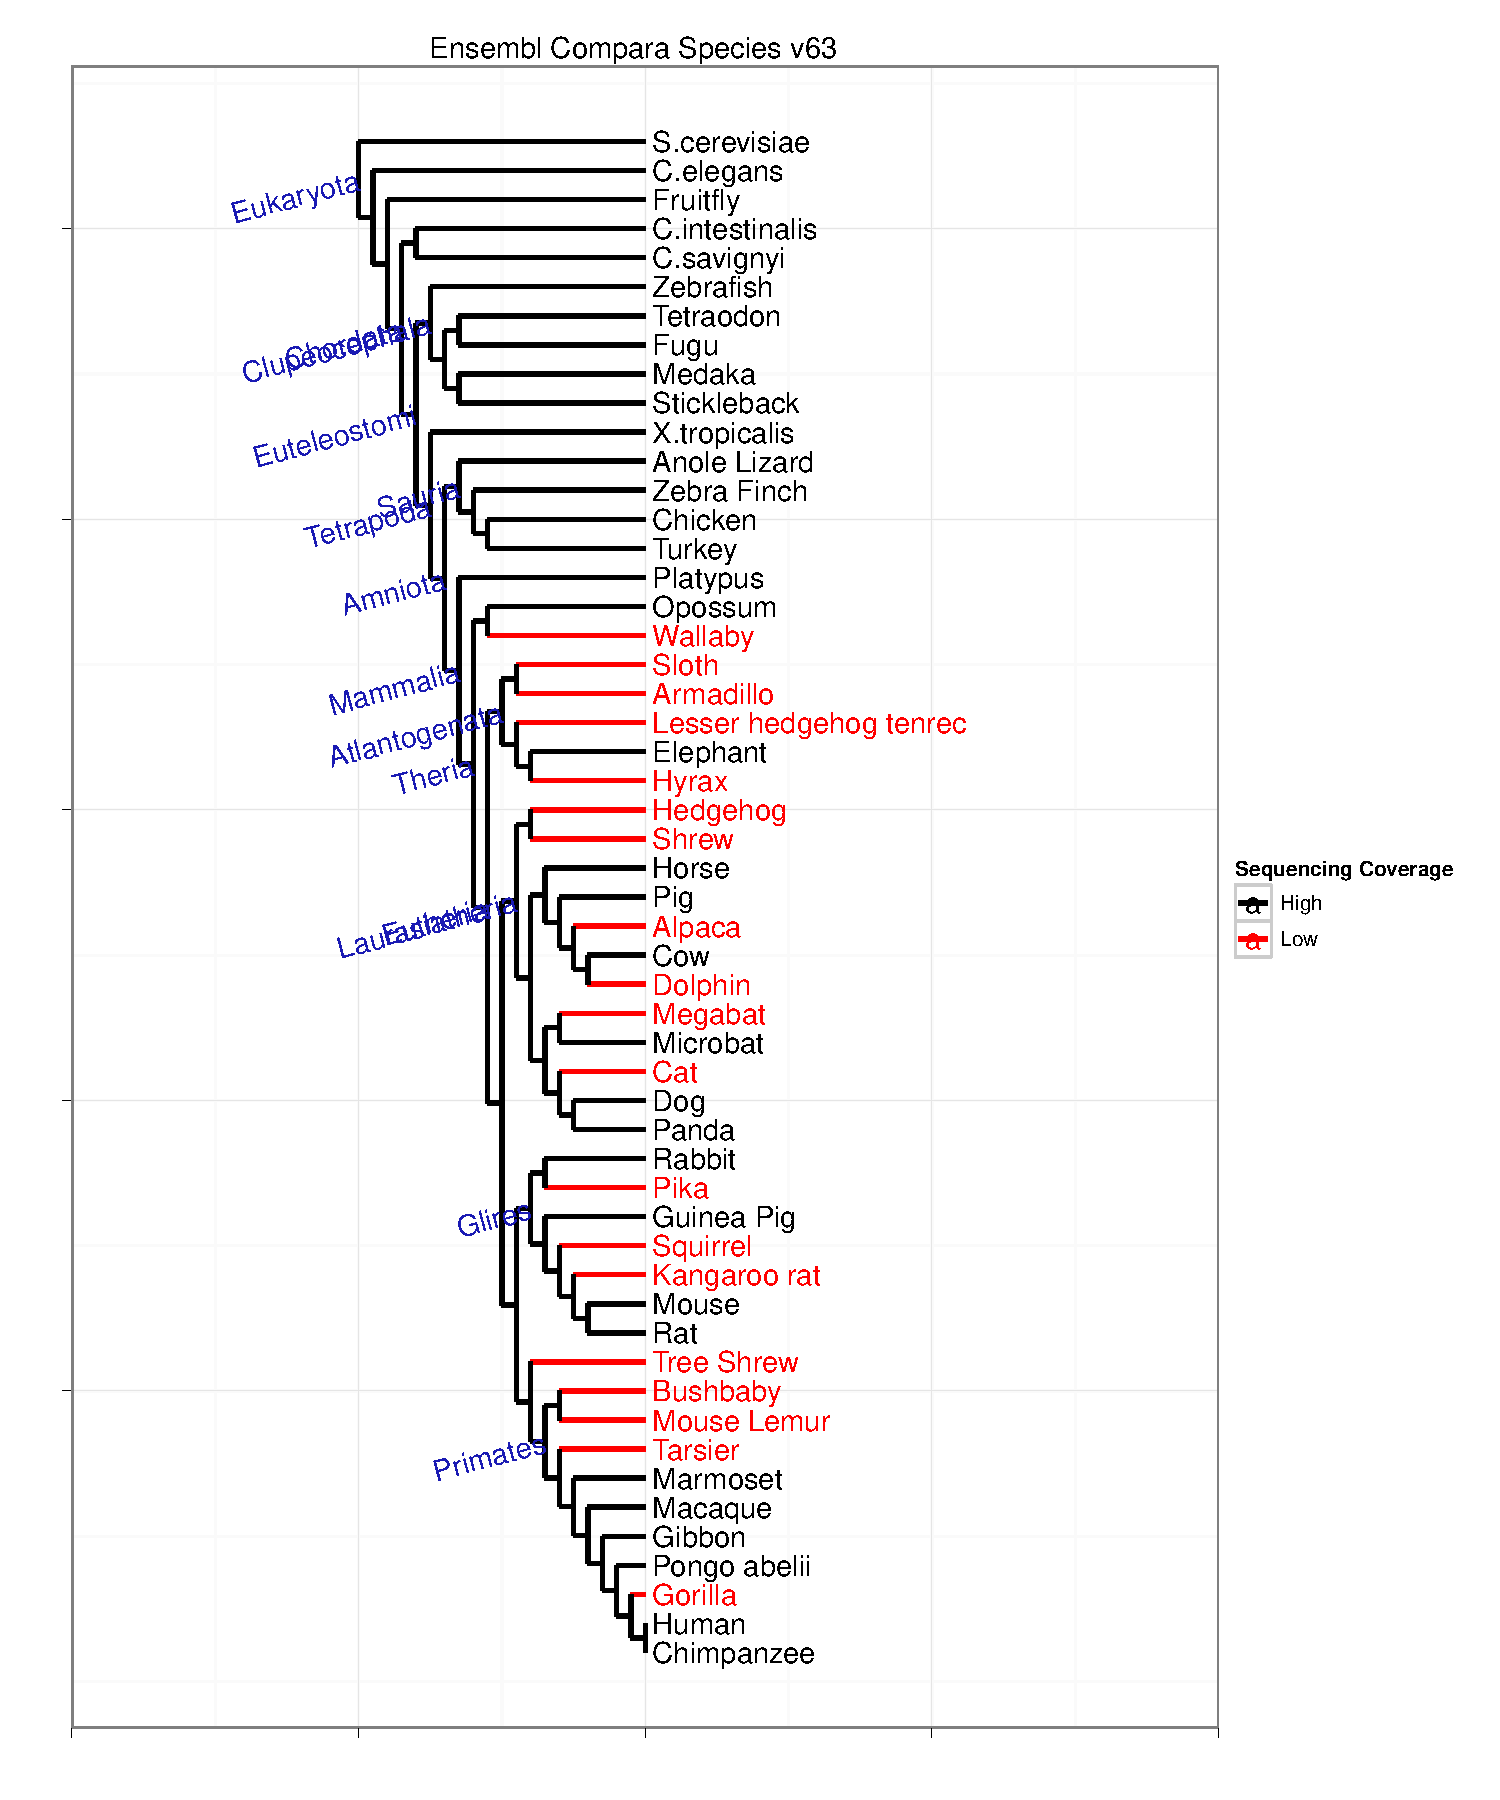
\includegraphics[scale=0.4]{Figs/compara_63_tree.pdf}
\caption{The NCBI taxonomy of species within the Ensembl Compara
  database. Note that branch lengths are not drawn to
  scale. Low-coverage genomes are labeled in red, high-coverage
  genomes are in black. Selected internal nodes, used are labeled in
  blue.}
\label{ncbi_tree}
\end{figure}


\begin{table}[h] \footnotesize
\centering
\begin{tabular}{@{}lll@{}} \toprule
\multicolumn{2}{c}{Method} \\ \cmidrule(r){1-2}
   Name & Category & Constraints \\ \midrule
   Primates & Ingroups & $TC(Primates) > 0.6$ \\
   Glires & &  $TC(Glires) > 0.6$ \\
   Laurasiatheria & & $TC(Laurasiatheria) > 0.6$ \\
   Sauria & & $TC(Sauria) > 0.6$ \\
   Fish & & $TC(Clupeocephala) > 0.6$ \\
   Eutheria & Outgroups & $TC(Eutheria) > 0.6$ \\
   Amniotes & & $TC(Amniota) > 0.6$\\
   Vertebrates & & $TC(Vertebrata) > 0.6$\\
   Fungi/Metazoa & & $TC(Fungi/Metazoa) > 0.6$\\
   MammalClades & & $TC_{all}(Laur., Glires, Primates) > 0.1$\\
   CladesPlusOutgroup &  & $TC_{all}(Laur., Glires, Primates) > 0.1$ AND \\
    & & $TC_{any}(Sauria, Clupeo., Ciona, Marsup.) > 0)$ \\
   Human Orthologs & Orthologs & \\
   Mouse Orthologs &  &  \\
   Zebrafish Orthologs &  &  \\
   Drosophila Orthologs &  &  \\
   Ensembl Roots & Root Nodes  &  \\
\bottomrule
\end{tabular}
\caption{Subtree constraints for identifying Eutherian orthologous
  subtrees. Ensembl gene trees were split into subtrees based on
  taxonomic coverage (TC) requirements at internal nodes, shown
  below. Laur. - Laurasiatheria; Clupeo. - Clupeocephala; Marsup. -
  Marsupiala}
\label{subtree_constraints}
\end{table}

\subsection{Analysis of genome-wide sets of orthologous mammalian trees}

The scheme described in the previous subsection was applied to the XYZ
root gene trees from the Ensembl database. Here I will describe the
resulting sets of trees and sub-trees, discuss what they reveal about
the evolutionary history of vertebrates and the feasibility of using
taxonomic coverage to isolate orthologous trees for sitewise analysis,
and finally, explain my reasoning for deciding to use the subtrees
based on the Eutherian taxonomic coverage for the subsequent sitewise
analysis.

First I will describe the set of root Compara gene trees, focusing on
their size and taxonomic coverage. I note that nearly half of all
Compara gene trees contain few sequences: 9,378 trees, over half of
the 18,607 root trees, constitute fewer than 20 sequences. Given the
protein-based clustering performed by the Compara pipeline, one might
expect many of these small trees to represent portions of larger
fast-evolving gene trees whose high sequence divergences made the
BLAST search step inaccurate or caused clustering via the \hclust
algorithm to be ineffective. Alternatively, these small clusters might
have resulted from exceptional lineage-specific gene duplications or
mis-annotated pseudogenes, causing a tight cluster of very
closely-related proteins that was identified by \hclust as an
independent cluster. Some evidence for the latter hypothesis comes
from the species counts and mean path lengths of the smaller versus
larger trees, shown in Table \ref{ensembl_root_table}. The subset of
small root trees has a median species count of 2 compared to 47 for
the large subset, indicating that most of the smaller trees encompass
sequences from a very small taxonomic range, and the median MPL for
the small trees is 0.04 compared to 1.04 for the large subset, showing
a much smaller average amount of sequence divergence. Together, these
summary statistics indicate that the smallest trees in the Compara
database consist of highly species-specific, closely-related proteins
that are likely artifactual gene annotations. In any case, Table
\ref{ensembl_root_table} shows that only a small fraction of human
genes---which we expect to be very well-annotated and to contain few
false positive genes due to the high level of manual curation and the
large amount of continued scrutiny---are contained within the smaller
trees (809 in total), indicating that whatever methodological artifact
or evolutionary process is causing the Compara pipeline to yield such
a high number of small gene trees, it has not had a significant impact
on the composition of the most confident set of protein-coding genes
within gene trees.

A closer examination of the distribution of tree sizes in the set of
root Compara trees clearly portrays the over-clustering
problem. Figure \ref{ensembl_roots_hist} shows the distribution of
sequence counts for all trees with more than 15 sequences, with
vertical dashed lines overlaid at each multiple of 48, the number of
vertebrate species in Ensembl release 63. The highest peak of the
histogram is at, or slightly above, 48 sequences, with the tree counts
quickly diminishing at larger sizes. Weaker, but still discernable,
peaks appear at larger tree sizes, however, with the location of these
echo-like peaks corresponding closely to the second, third and fourth
multiple of 48 sequences. Beyond the level of 200 sequences, the peaks
become indistinguishable, but there is still a long tail of rather
large trees extending out to a maximum size of 400 sequences. This
distribution is consistent with the situation I described above,
whereby the Compara pipeline clusters together multiple
largely-orthologous gene trees. The peaks become smaller and more
diffuse at larger sequence counts because larger trees have more chance of 



\begin{table}[hb] \footnotesize
\centering
\begin{tabular}{lb{3cm}rrrrb{1cm}b{1cm}}
\toprule
Tree Set & Med. Size & \multicolumn{3}{c}{\% w/ Human Count} & Human & Med. & Med. \\ \cmidrule(r){3-5}
  & (Min / Max) & 0 & 1 & 2+ & Total & MPL & Species \\ 
  \midrule
Ensembl Roots & 15 (2 / 400) & 0.50 & 0.30 & 0.20 & 19995 & 0.55 & 8 \\ 
($<$= 15) & 3 (2 / 15) & 0.92 & 0.08 & 0.00 & 809 & 0.04 & 2 \\ 
($>$ 15) & 54 (16 / 400) & 0.07 & 0.53 & 0.40 & 19186 & 1.04 & 47 \\ 
   \bottomrule
\end{tabular}
\caption{Summary of the set of Ensembl Compara root trees. The columns
  under '\% Human Count' represent the percentage of trees which
  contain the indicated number of human genes. 'Med. Species' is the
  median species count across all trees. Med. - median, MPL - mean
  path length }
\label{ensembl_root_table}
\end{table}


\begin{figure}[t]
\centering
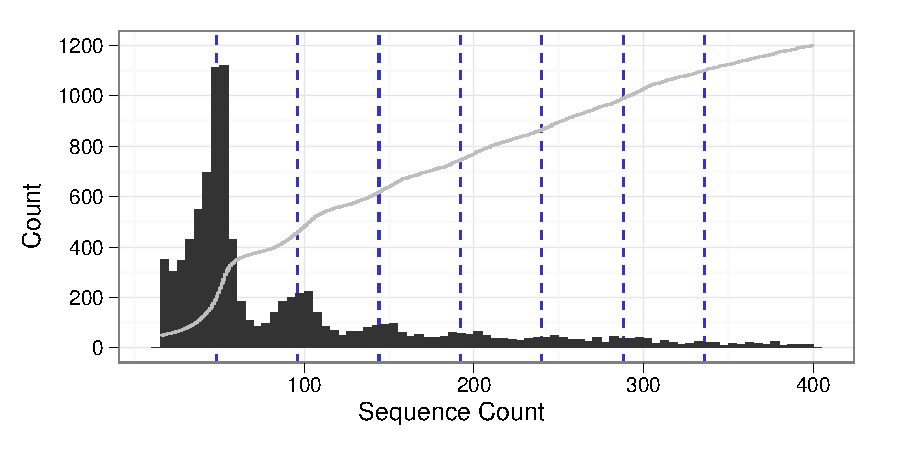
\includegraphics[scale=0.9]{Figs/ensembl_roots_hist.pdf}
\caption{Gene tree sizes for the root Compara trees. Trees with fewer
  than 15 sequences (n=9,378) are not shown for the purpose of
  clarity; the remaining 9,229 trees are shown in bins of width
  5. Dashed green lines are drawn at integral multiples (from 1 to 5)
  of the number of vertebrate species within Ensembl (n=48).}
\label{ensembl_roots_hist}
\end{figure}


%\subsection{Filtering out low-quality genome sequence}

%\subsection{Realigning coding sequences}

%For example, coding sequence
%alignments are generated by the Compara pipeline as a necessary
%intermediate result, but these alignments are neither designed nor
%quality-controlled for use in detailed sitewise evolutionary
%analyses. In light of my results from Chapter XYZ regarding the
%tendency of different aligners to produce false positive results in sitewise analyses, 

%\subsection{Filtering out clusters of \nsyn substitutions}

%\section{Results}


%\subsection{Analysis of the global distribution of mammalian selective pressures}



%\subsection{Analysis of sitewise estimates from three mammalian sub-clades}



%\subsection{Evaluation of the effect of GC content, recombination rate, and codon usage on sitewise dnds estimates and the detection of positive selection}


%\section{Conclusions}

